\chapter{Proposed Algorithm}
\label{chap:algorithm}

\section{Recap: Alternating Optimization with Genetic Algorithm and Simulated Annealing (GASA)}

Alternating optimization is a widely used strategy for non-convex problems that involve multiple variables or mixed types of parameters. The core idea is to decompose the original challenging joint optimization into two or more easier subproblems, which are solved iteratively. In our problem, we first fix the power allocation $P$ and optimize the SSB periodicity $\theta$. Then, we fix the SSB periodicity $\theta$ and optimize the power allocation $P$. This process repeats until convergence. Thus, the problem (\ref{eq:main}) can be devided to two subproblems. 

\subsection{Fix Power Optimize SSB Periodicity}

\begin{subequations} \label{eq:FPOS}
\begin{align}
    &\min_{\theta} \sum_{u} \sum_{\mathcal{S}_i\in \mathcal{\widetilde{S}}} \mathbb{E}[\alpha_u[\mathcal{S}_i]] \\ 
    &\text{subject to} \nonumber \\
    &\theta_k[\mathcal{S}_i] \leq N, \quad \forall k\in\mathcal{K}, \mathcal{S}_i\in\mathcal{\widetilde{S}} \\
    &\theta_k[\mathcal{S}_i] \in \mathbb{N}^+, \quad \forall k\in\mathcal{K}, \mathcal{S}_i\in\mathcal{\widetilde{S}} \\
    &\sum_k \frac{1}{\theta_k[\mathcal{S}_i]} \leq M, \quad \forall \mathcal{S}_i\in\mathcal{\widetilde{S}}
\end{align}
\end{subequations}

We use Genetic Algorithm to solve this problem:

\begin{algorithm}[H]
    \caption{Fix Power, Optimize SSB Periodicity}
    \label{alg:FPOS}
    \begin{algorithmic}[1]
        \REQUIRE{}
        Given the transmission power $P_{k, \mathcal{S}_i}$ for each cell $k$ at each epoch $\mathcal{S}_i$, as well as the user distribution.
        \ENSURE
        Find and assign the optimal SSB periodicity $\theta_{k,\mathcal{S}_i}$ for each cell, such that the user access delay is minimized while the periodicity configuration for all cells meets the available resource constraints.
        % \FOR{every epoch $\mathcal{S}_i$}
        % \STATE initialize the SSB periodicity $\theta_{k,\mathcal{S}_i}$ for all cells $k$. 
        % \STATE Compute the expected random access delay $\mathbb{E}[\alpha_u[s]]$ for each UE. 
        % \STATE According to the periodicity formulas (3.7~3.11), combine transmission power, path loss, and antenna gain to calculate the success probability of SSB reception for each cell.
        % \STATE Continuously adjust $\theta_{k,\mathcal{S}_i}$ such that the delay and the resource constraint are satisfied.
        % \STATE Finally, obtain the periodicity allocation that yields the minimum delay.
        % \ENDFOR
        \STATE Generate initial population of candidate solutions with size $POP\_SIZE$.
        \STATE Each individual is a vector of integers $\theta_k[\mathcal{S}_i]$ within constraints. 
        \FOR{generation = 1 to max\_generations}
            \FOR{each individual in population}
                \STATE Compute $\mathbb{E}[\alpha_u[\mathcal{S}_i]]$ by (3.7)-(3.11)
                \STATE Assign fitness = $1 / \mathbb{E}[\alpha_u[\mathcal{S}_i]]$
            \ENDFOR
            \STATE Select parents based on fitness
            \STATE Apply crossover to produce offspring
            \STATE Apply mutation to offspring within constraints
            \STATE Calculate fitness for offspring
            \STATE Select next generation population from parents and offspring
        \ENDFOR
        \STATE \textbf{return} individual with best fitness as optimal periodicity vector
    \end{algorithmic}
\end{algorithm}

\subsection{Fix SSB Periodicity Optimize Power}

\begin{subequations}
\begin{align}
    &\min_{P} \sum_{u} \sum_{\mathcal{S}_i\in \mathcal{\widetilde{S}}} \mathbb{E}[\alpha_u[\mathcal{S}_i]] \\
    &\sum_{m} \frac{P_{k}[\mathcal{S}_i]}{\theta_k[\mathcal{S}_i]} \leq P^{total}, \quad \forall \mathcal{S}_i \in \mathcal{\widetilde{S}}  \\ 
    &P_k[\mathcal{S}_i]\geq 0, \quad \forall k\in\mathcal{K}, \mathcal{S}_i\in\mathcal{\widetilde{S}}
\end{align}
\end{subequations}

We use Simulated Annealing to solve this problem:

\begin{algorithm}[H]
    \caption{Fix SSB Periodicity, Optimize Power}
    \label{alg:FSOP}
    \begin{algorithmic}[1]
        \REQUIRE{}
        Given the transmission power $\theta_{k,\mathcal{S}_i}$ for each cell $k$ at each epoch $\mathcal{S}_i$, as well as the user distribution.
        \ENSURE
        Find and assign the optimal SSB periodicity $P_{k, \mathcal{S}_i}$ for each cell, such that the user access delay is minimized while the periodicity configuration for all cells meets the available resource constraints.
        % \FOR{every epoch $\mathcal{S}_i$}
        % \STATE initialize the transmit power $P_{k, \mathcal{S}_i}$ for all cells $k$. 
        % \STATE Compute the expected random access delay $\mathbb{E}[\alpha_u[s]]$ for each UE. 
        % \STATE According to the periodicity formulas (3.7~3.11), combine transmission power, path loss, and antenna gain to calculate the success probability of SSB reception for each cell.
        % \STATE Continuously adjust $P_{k, \mathcal{S}_i}$ such that the delay and the resource constraint are satisfied.
        % \STATE Finally, obtain the power allocation that yields the minimum delay.
        % \ENDFOR
        
        % \STATE \textbf{Input:} Fixed SSB periodicity $\text{Periodicity} = \{period_k\}$ for cells $k=1 \dots K$
        \STATE Initialize current solution $P_{current}$ with feasible power allocation
        \STATE Calculate $current\_delay$ $\mathbb{E}[\alpha_u[\mathcal{S}_i]]$ for $P_{current}$
        \STATE Initialize temperature $T \gets T_{max}$, cooling rate $0 < \alpha < 1$
        \WHILE{$T > T_{min}$}
            \STATE Generate new solution $P_{new}$ by perturbing $P_{current}$ within constraints
            \STATE Calculate $new\_delay$ for $P_{new}$
            \IF{$new\_delay < current\_delay$}
                \STATE Accept $P_{new}$: $P_{current} \gets P_{new}$, $current\_delay \gets new\_delay$
            \ELSE
                \STATE Accept $P_{new}$ with probability $\exp\left(-\frac{new\_delay - current\_delay}{T}\right)$
            \ENDIF
            \STATE Update temperature $T \gets \alpha \times T$
        \ENDWHILE
        \STATE \textbf{return} $P_{current}$ as optimized power allocation
    \end{algorithmic}
\end{algorithm}

\begin{figure}[h!]
    \centering
    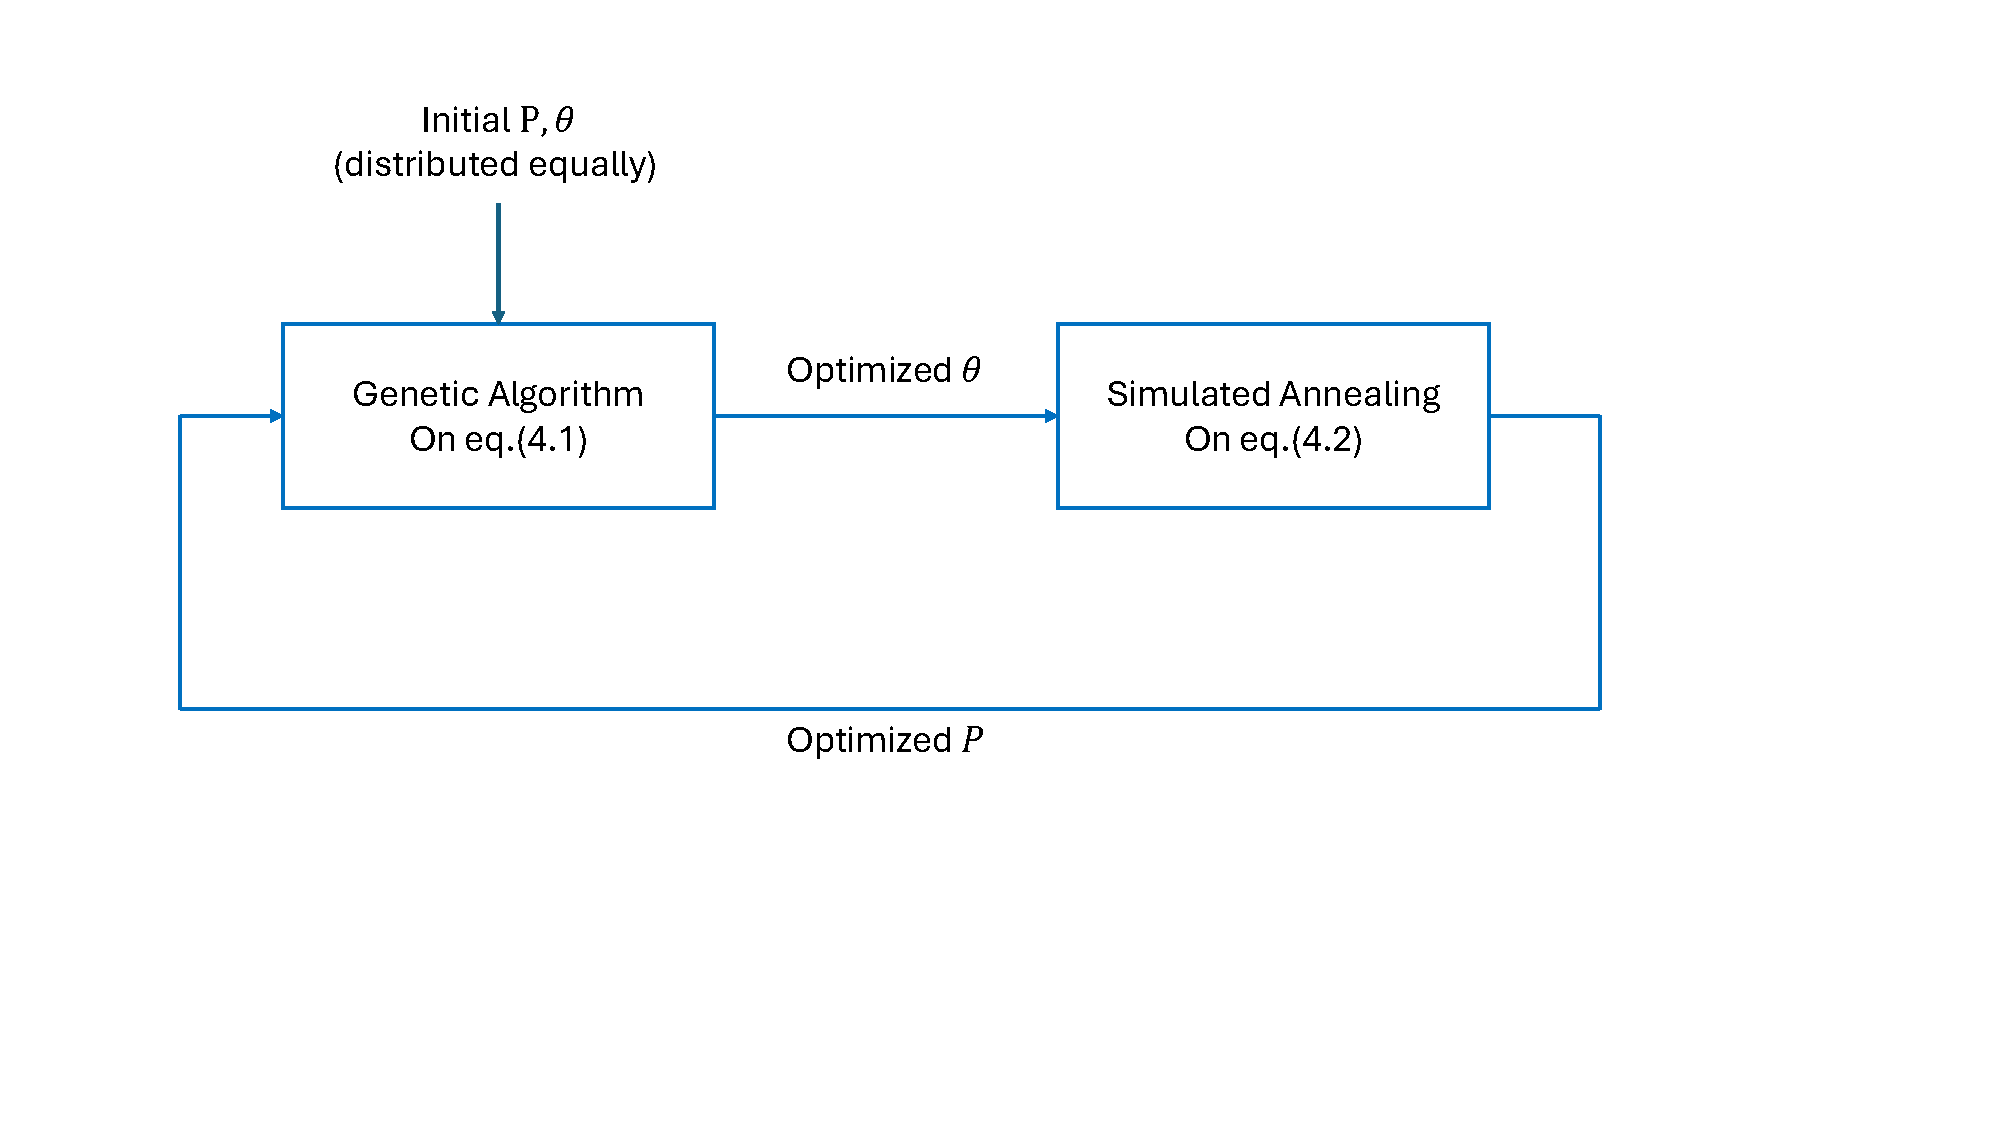
\includegraphics[width=1\textwidth]{figure/GASA.pdf}
    \caption{GASA diagram flow}
    \label{GASA diagram flow}
\end{figure}

\begin{figure}[h!]
    \centering
    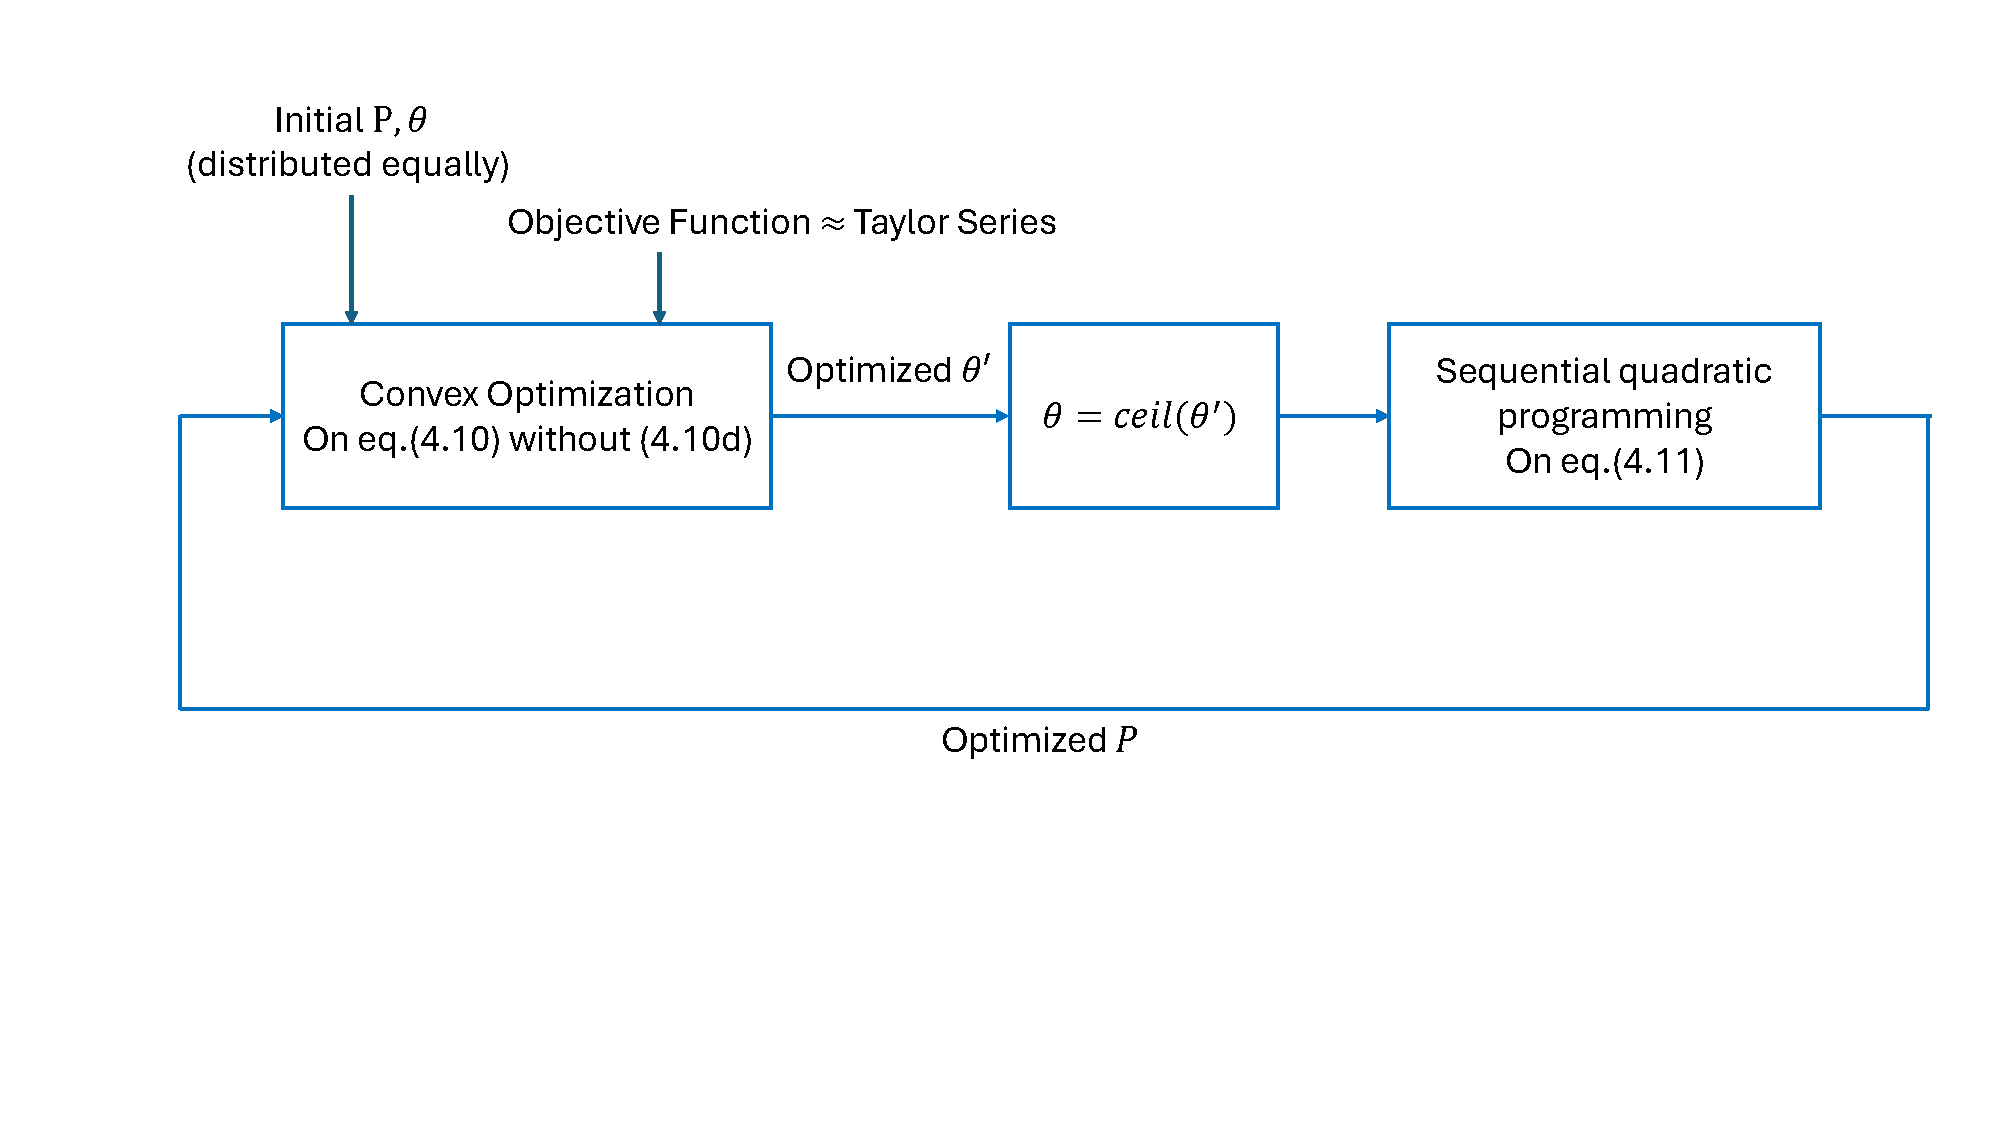
\includegraphics[width=1\textwidth]{figure/Taylor.pdf}
    \caption{Taylor series expansion diagram flow}
    \label{Taylor diagram flow}
\end{figure}

\section{Taylor Expansion on Objective Function}

In this method, we use Taylor expansion on $F_{h_k}$ to approximate the non-linear term into linear term. Below are the calculations:
\begin{equation}
    F(x) = K \sum_{n=0}^\infty \frac{(m)_n d^n (2b)^{tn}}{(n!)^2} \zeta(1+n, \frac{x}{2b})
\end{equation}
\begin{equation}
    F'(x) = K \sum_{n=0}^\infty \frac{(m)_n d^n (2b)^{tn}}{(n!)^2} \left( \frac{x}{2b} \right)^n e^{\frac{x}{2b}} \cdot \frac{1}{2b}
\end{equation}
Given a real number $a$, the first order Taylor series of a real function $f(x)$ can be expressed as:
\begin{equation}
    \begin{aligned}
        f(x) &\approx f(a) + f'(a)\cdot(x-a)
    \end{aligned}
\end{equation}
Then the expectation of the number of SSB reception failures $Q_u[S_i]$ can be expressed as follows:
\begin{equation}
    \begin{aligned}
        &\mathbb{E}[Q_u[S_i]] = \frac{F\left( \frac{P_k^{\text{th}}}{P_k \cdot L_k} \right)}{1 - F\left( \frac{P_k^{\text{th}}}{P_k \cdot L_k} \right)} \\
        &\approx \frac{F(a) + F'(a) \cdot \left( \frac{P_k^{\text{th}}}{P_k \cdot L_k} - a \right)}{1 - \left[ F(a) + F'(a) \cdot \left( \frac{P_k^{\text{th}}}{P_k \cdot L_k} - a \right) \right]}
    \end{aligned}
\end{equation}
where $k$ is the cell that the $u$-th user connected to. The expectation of user cell searching delay can be expressed as follows:
\begin{equation}
    E[\alpha_u] = E[\beta_u] + E[\gamma_u]
    =\left( \frac{1}{2} + \frac{P_k C + E_k}{P_k (1-C) - E_k} \right) \theta_k
\end{equation}
where $C = F(a) - F'(a)\cdot a$, $E_k = \frac{F'(a) P^{th}}{L_k}$. We introduce the population density of the $k$-th cell as $D_k$. Then the cell searching delay for all UE can expressed as follows:
\begin{equation}
    \sum_u E[\alpha_u] = \sum_k D_k \left( \frac{1}{2} + \frac{P_k C + E_k}{P_k (1-C) - E_k} \right) \theta_k
\end{equation}
We can rewrite the problem from \ref{eq:main} as follows:
\begin{subequations} \label{eq:taylor}
    \begin{align}
        &\min_{P, \theta} \frac{1}{\sum_k D_k}\sum_k D_k \left( \frac{1}{2} + \frac{P_k C + E_k}{P_k (1-C) - E_k} \right) \theta_k \\
        &\text{subject to} \\
        &\quad P_k > 0, \quad \forall k \in \mathcal{K} \\
        &\quad \theta_k \leq N, \quad \forall k \in \mathcal{K} \\
        &\quad \theta_k \in \mathbb{N}^+, \quad \forall k \in \mathcal{K} \\
        &\quad \sum_k P_k \leq P_{\text{total}} \\
        &\quad \sum_k \frac{1}{\theta_k} \leq M
    \end{align}
\end{subequations}
We use alternating optimization to seperate equation (\ref{eq:taylor}) into two subproblems. With fixed power, we optimize SSB periodicity:
\begin{subequations} \label{taylor_theta}
    \begin{align}
        &\min_{\theta} \frac{1}{\sum_k D_k}\sum_k D_k \left( \frac{1}{2} + \frac{P_k C + E_k}{P_k(1-C) - E_k} \right) \theta_k \\
        &\text{subject to} \\
        &\quad \theta_k \leq N, \quad \forall k \in \mathcal{K} \\
        &\quad \theta_k \in \mathbb{N}^+, \quad \forall k \in \mathcal{K} \\
        &\quad \sum_k \frac{P_k}{\theta_k} \leq P_{\text{total}} \\
        &\quad \sum_k \frac{1}{\theta_k} \leq M
    \end{align}
\end{subequations}
And with fixed SSB periodicity, we optimize power:
\begin{subequations} \label{taylor_power}
    \begin{align}
        &\min_{P} \frac{1}{\sum_k D_k}\sum_k D_k \left( \frac{1}{2} + \frac{P_k C + E_k}{P_k(1-C) - E_k} \right) \theta_k \\
        &\text{subject to} \\
        &\quad P_k > 0, \quad \forall k \in \mathcal{K} \\
        &\quad \sum_k \frac{P_k}{\theta_k} \leq P_{\text{total}}
    \end{align}
\end{subequations}

For problem (\ref{taylor_theta}), it satisfies convex optimization problem if we ignore constraint (\ref{taylor_theta}d). Thus, we compute the problem (\ref{taylor_theta}) without constraint (\ref{taylor_theta}d) by cvx in matlab, and then ceil the $\theta$ to make sure all $\theta$ satisfy constraint (\ref{taylor_theta}d). 

For problem (\ref{taylor_power}), it is not a convex optimization problem. Thus I use sequential quadratic programming (SQP) to calculate the result. 

\section{Result}
The result is shown in Table 1. We distribute power and SSB periodicity for all cells as our baseline. That is, 
\begin{equation}
    P_k = P_{total} / M, \quad \forall k \in \mathcal{K}
\end{equation}
\begin{equation}
    \theta_k = K / M, \quad \forall k \in \mathcal{K}
\end{equation}
The result of GASA is not quite well. The gain is calculated as $\frac{(\text{delay of baseline} - \text{delay of proposed method})}{\text{delay of baseline}}$. The average delay is not better than baseline and it does not converge through iteration, as shown in Figure 5. The result of Taylor expansion is better than baseline. 

\begin{table}[h!]
\centering
\caption{Comparison of different solution method}
\begin{tabular}{|c|c|c|c|}
\hline
    & Equally Distributed & GASA & Taylor \\
\hline
delay (number of time slots) & 18.6805 & 21.9090 & 13.6312 \\
\hline
gain & 0\% & -17\% & 27\% \\
\hline
\end{tabular}
\end{table}

\begin{figure}[h!]
    \centering
    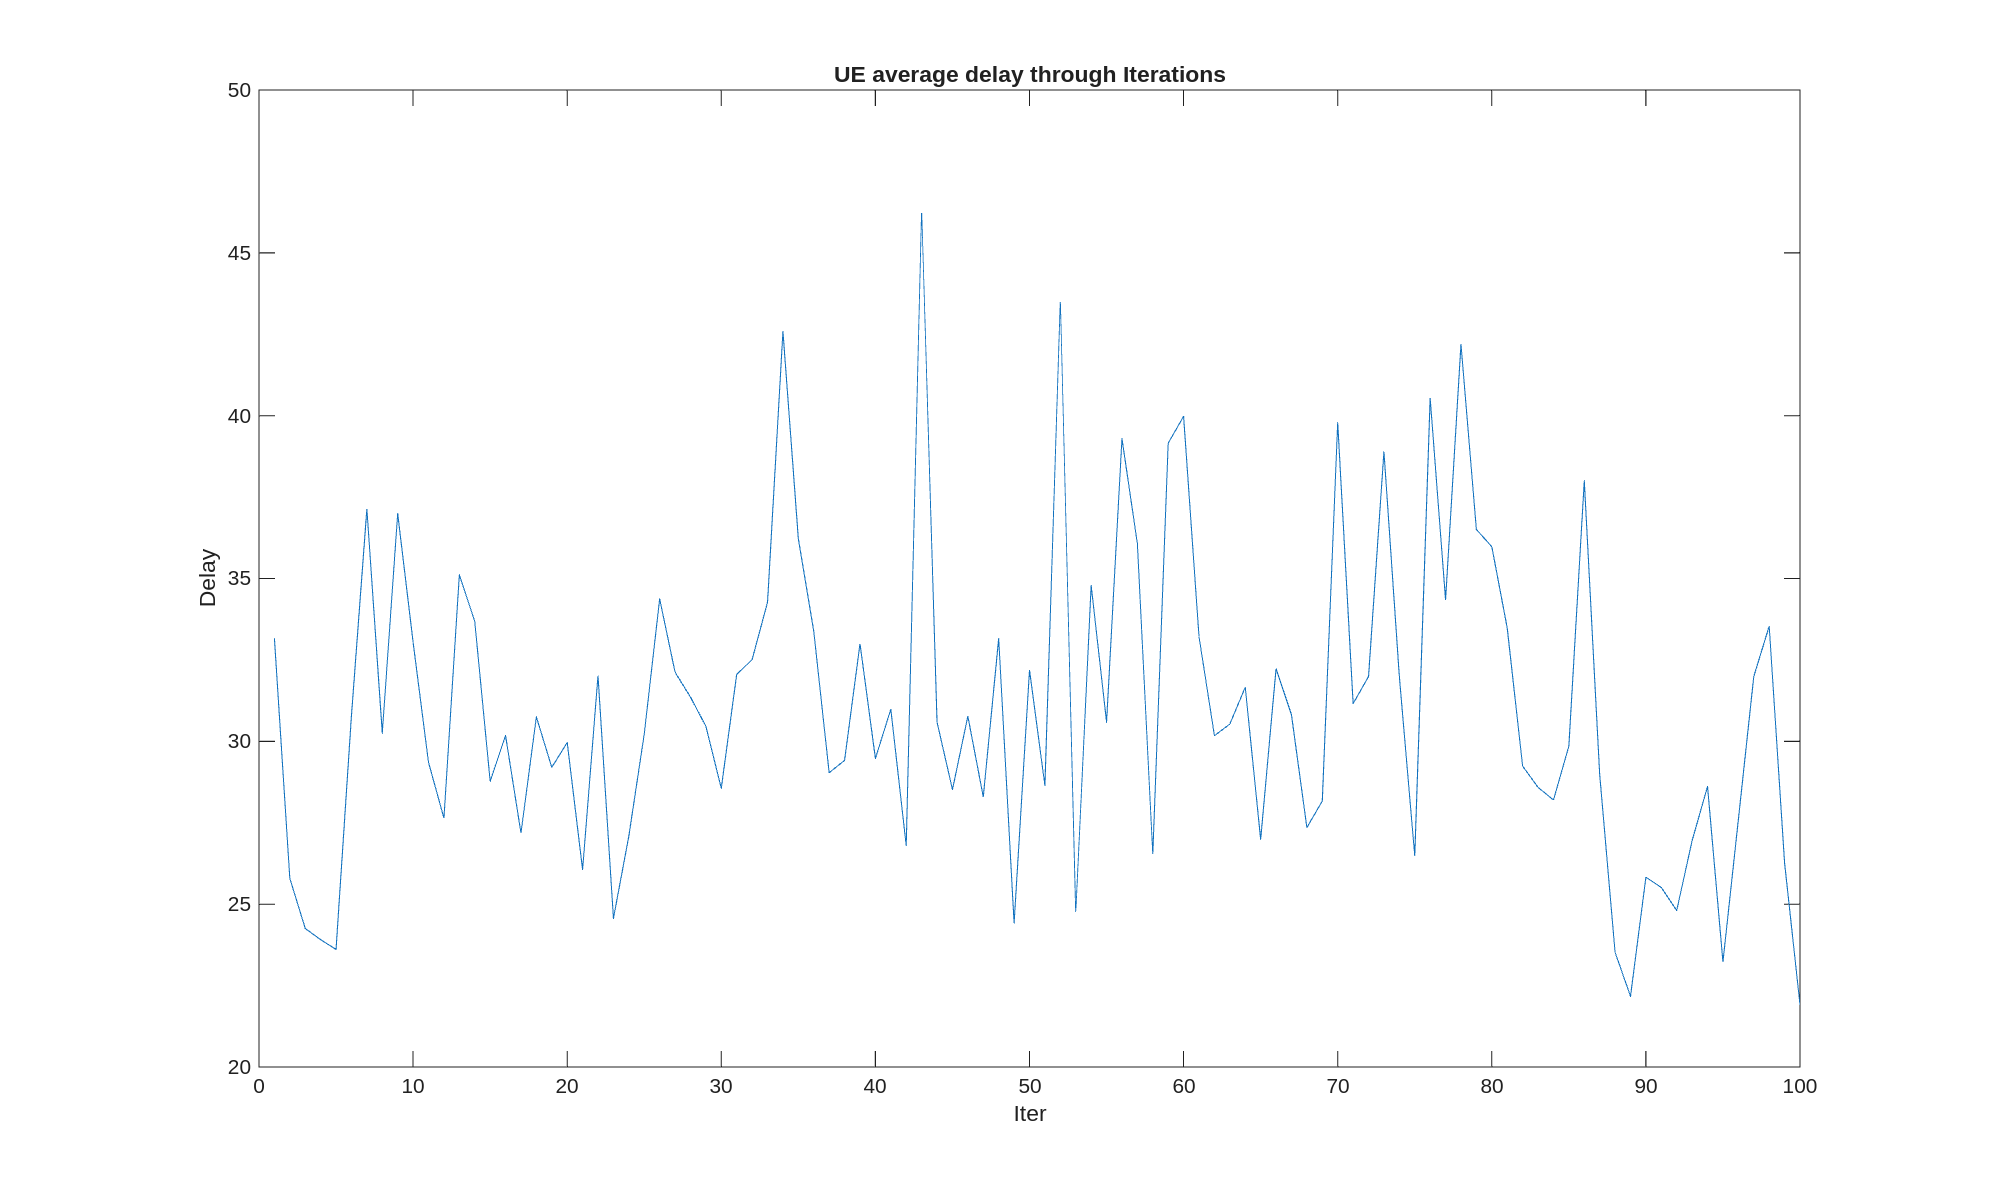
\includegraphics[width=1\textwidth]{thesis_code/result_GASA.png}
    \caption{Average delay of GASA through iterations.}
    \label{GASA iteration}
\end{figure}

\section{Future Work}
\begin{enumerate}
    \item I have found the reason why GASA has bad result. I will modify it and compare the result with other methods.
    \item To solve equation (4.11), maybe Dinkelbach algorithm can work.
    \item I am still figuring out how to determine $a$ in Taylor series.
    \item I only consider one epoch in the algorithm above. The relation between different epochs still need to be considered. 
\end{enumerate}